%\section{Introducción a la Modulación digital pasabanda}

Hasta ahora vimos transmisión de símbolos digitales por pulsos de
banda base, que son apropiados para canales que responden en esas
frecuencias. Por ejemplo, el par trenzado o cable coaxial, usado
en líneas T1 de telefonía.

Muchas veces, hace falta modular datos digitales en otras partes del espectro, por ejemplo:
\begin{enumerate}
    \item Modems para el canal telefónico de voz, que no responde en continua.
    \item Enlaces de radio microondas entre dos torres
    \item Telefonia celular.
\end{enumerate}

\noindent En principio, una solución posible sería modular en
forma analógica una onda digital de banda base:

\begin{figure}[htb]
    \centering\begin{minipage}{\textwidth}
    \bpgf{Imagenes/MDPasa/MDPasa-1}
    \begin{blockdiagram}
        \matrix[row sep=5mm, column sep=10mm]{
            \node[etiqueta] (inicio) {\parbox{2cm}{\centering fuente digital\\$\{a_k\}$}}; & \node [block] (modD) {\parbox{2cm}{MODUL\\DIGITAL}}; & \node [block] (modA) {\parbox{2cm}{MODUL\\ANALOG.}};\\
            & & & \node [block] (canal) {\parbox{2.5cm}{\centering CANAL\\PASABANDA}};\\
            \node[punto] (salida) {}; &\node [block] (detD) {\parbox{2.5cm}{DETECCIÓN\\DIGITAL}}; & \node[block] (detA) {\parbox{2cm}{DEMOD.\\ANALOG.}};\\
        };
        \draw [->] (inicio) -- (modD);
        \draw [->] (modD) -- node [below=12mm] {$\sum a_k p(t-kT_s)$} (modA);
        \draw [->] (modA) -| (canal);
        \draw [->] (canal) |- (detA);
        \draw [->] (detA) -- (detD);
        \draw [->] (detD) -- (salida);
    \end{blockdiagram}
    \endpgfgraphicnamed\end{minipage}
\end{figure}
\FloatBarrier

Esto es conceptualmente correcto, pero no necesariamente lo más eficiente. Puede
convenir combinar los bloques de arriba y los de abajo, aprovechando el hecho de que transmito señales ``especiales'' de
banda base. En particular para la detección, el objetivo es identificar el símbolo enviado, para cual no hace
falta demodular fielmente la onda analógica intermedia de banda base.

Para la modulación, esto implica generar directamente una señal
similar a la PAM, pero donde los pulsos de banda base $p(t)$ son
reemplazados por {\em pulsos de radiofrecuencia}, concentrados en
la banda de interés para la comunicación.

\newpage

Las siguientes figuras muestran ejemplos de este tipo, en comparación con el caso de banda base.
En cada caso, la amplitud (ASK), fase (PSK) o frecuencia (FSK) del pulso se utiliza para codificar el
símbolo, que en estos casos es binario.

\begin{figure}[htb]
    \centering
    \resizebox{\textwidth}{!}{
    \bpgf{Imagenes/MDPasa/MDPasa-2}
    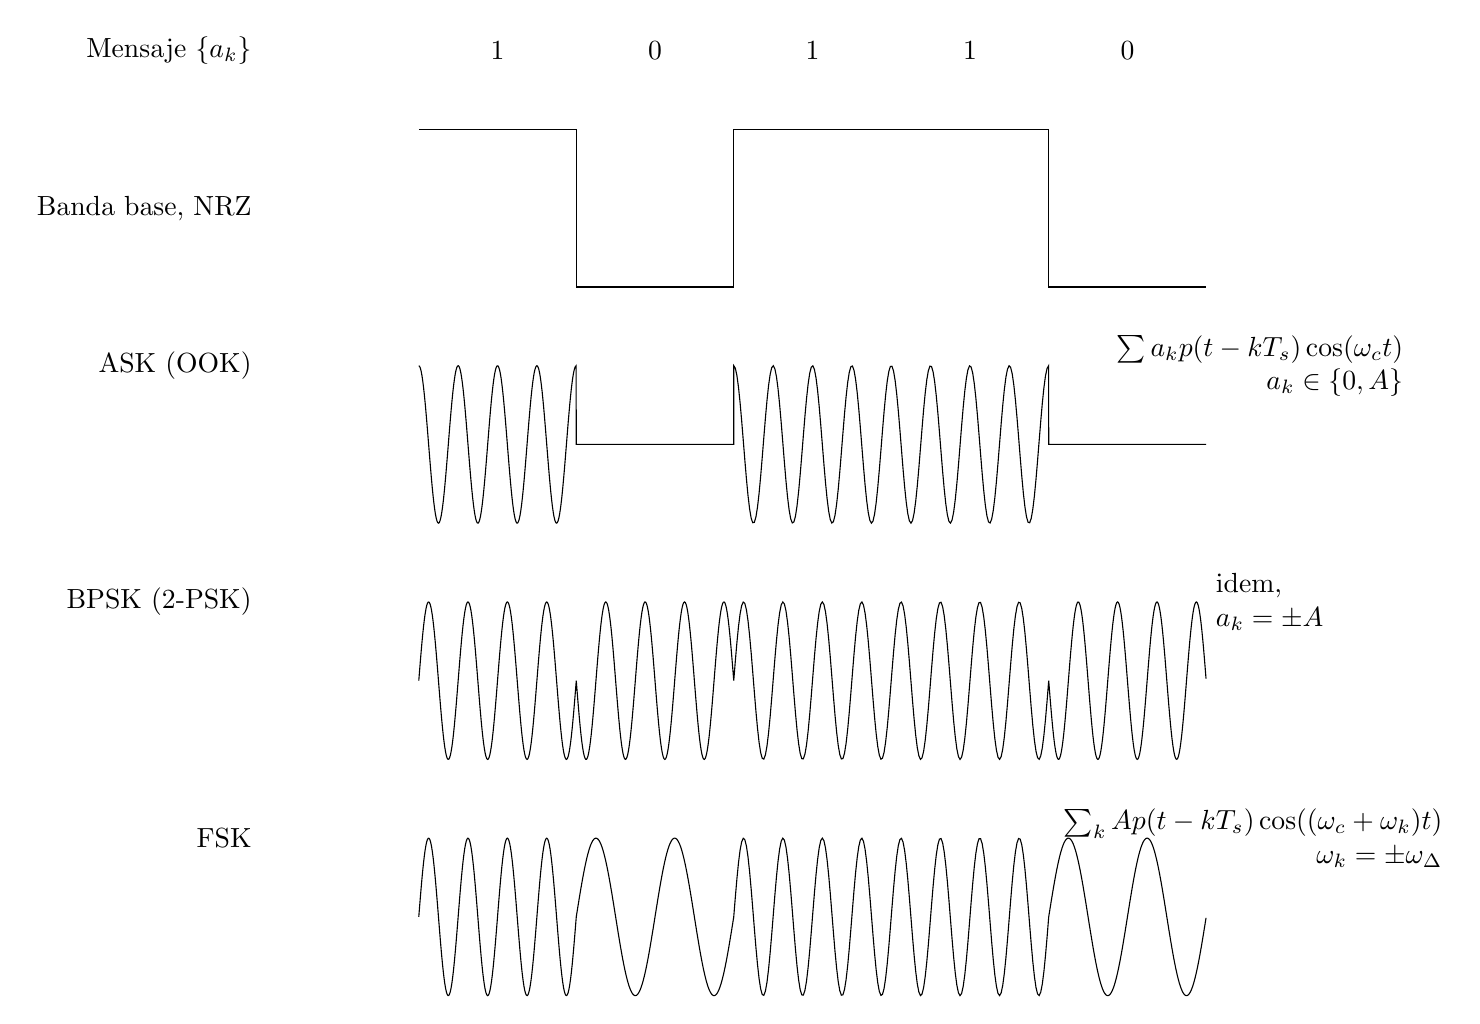
\begin{tikzpicture}
        \path (-2,1) node [anchor=east] {Mensaje $\{a_k\}$};
        \path (1,1) node {$1$} -- (3,1) node {$0$} -- (5,1) node {$1$} -- (7,1) node {$1$} -- (9,1) node {$0$};
        \begin{scope}[shift={(0,-2)}]
            \path (-2,1) node [anchor=east] {Banda base, NRZ};
            \draw (0,2) -- (2,2) -- (2,0) -- (4,0) -- (4,2) -- (8,2) -- (8,0) -- (10,0);
        \end{scope}
        \begin{scope}[shift={(0,-4)}]
            \path (-2,1) node [anchor=east] {ASK (OOK)};
            \draw [samples=200,domain=0:2] plot (\x,{cos(4*pi*\x r)}) -- (2,0) -- (4,0) -- plot [samples=200,domain=4:8] (\x,{cos(4*pi*\x r)}) -- (8,0) -- (10,0);
            \path (10,1) node {\parbox{5cm} {\raggedleft $\sum a_k p(t-kT_s)\cos(\omega_ct)$\\$a_k\in\{0,A\}$}};
        \end{scope}
        \begin{scope}[shift={(0,-7)}]
            \path (-2,1) node [anchor=east] {BPSK (2-PSK)};
            \draw [samples=200,domain=0:2] plot (\x,{sin(4*pi*\x r)}) -- plot [domain=2:4] (\x,{-sin(4*pi*\x r)}) -- plot [samples=200,domain=4:8] (\x,{sin(4*pi*\x r)}) -- plot [domain=8:10] (\x,{-sin(4*pi*\x r)});
            \path (10,1) node [anchor=west] {\parbox{2.5cm}{idem,\\$a_k = \pm A$}};
        \end{scope}
       \begin{scope}[shift={(0,-10)}]
            \path (-2,1) node [anchor=east] {FSK};
            \draw [samples=200,domain=0:2] plot (\x,{sin(4*pi*\x r)}) -- plot [domain=2:4] (\x,{sin(2*pi*\x r)}) -- plot [samples=200,domain=4:8] (\x,{sin(4*pi*\x r)}) -- plot [domain=8:10] (\x,{sin(2*pi*\x r)});
%            \path (10,1) node [anchor=west] {\parbox{2.5cm}{fórmula\\después}};
            \path (10,1) node {\parbox{6cm}{\raggedleft $\sum_k A p(t-kT_s) \cos ((\omega_c  + \omega_k) t)$ \\ $\omega_k = \pm \omega_\Delta$ }};
        \end{scope}
    \end{tikzpicture}
    \endpgfgraphicnamed
    }
\end{figure}
\FloatBarrier
%
Los casos de ASK y BPSK corresponden a modulación lineal, es decir
que $x_c$ depende linealmente de los símbolos; en el caso de FSK la dependencia es no lineal.
En los dibujos se utilizó $p(t)$ rectangular, NRZ; también puede pensarse en modular pulsos de
banda base más sofisticados, como los de Nyquist (más dificiles de
dibujar en el tiempo). 